\documentclass{ximera}

%\usepackage{todonotes}

\newcommand{\todo}{}

\usepackage{tkz-euclide}
\tikzset{>=stealth} %% cool arrow head
\tikzset{shorten <>/.style={ shorten >=#1, shorten <=#1 } } %% allows shorter vectors

\usepackage{tkz-tab}  %% sign charts
\usetikzlibrary{decorations.pathreplacing} 

\usetikzlibrary{backgrounds} %% for boxes around graphs
\usetikzlibrary{shapes,positioning}  %% Clouds and stars
\usetikzlibrary{matrix} %% for matrix
\usepgfplotslibrary{polar} %% for polar plots
\usetkzobj{all}
\usepackage[makeroom]{cancel} %% for strike outs
%\usepackage{mathtools} %% for pretty underbrace % Breaks Ximera
\usepackage{multicol}

\usepackage{polynom}



\usepackage[many]{tcolorbox}  %% for titled boxes
\newtcolorbox{xbox}[1]{%
    tikznode boxed title,
    enhanced,
    arc=0mm,
    interior style={white},
    attach boxed title to top center= {yshift=-\tcboxedtitleheight/2},
    fonttitle=\bfseries,
    colbacktitle=white,coltitle=black,
    boxed title style={size=normal,colframe=white,boxrule=0pt},
    title={#1}}


\usepackage{array}
\setlength{\extrarowheight}{+.1cm}   
\newdimen\digitwidth
\settowidth\digitwidth{9}
\def\divrule#1#2{
\noalign{\moveright#1\digitwidth
\vbox{\hrule width#2\digitwidth}}}





\newcommand{\RR}{\mathbb R}
\newcommand{\R}{\mathbb R}
\newcommand{\N}{\mathbb N}
\newcommand{\Z}{\mathbb Z}

%\renewcommand{\d}{\,d\!}
\renewcommand{\d}{\mathop{}\!d}
\newcommand{\dd}[2][]{\frac{\d #1}{\d #2}}
\newcommand{\pp}[2][]{\frac{\partial #1}{\partial #2}}
\renewcommand{\l}{\ell}
\newcommand{\ddx}{\frac{d}{\d x}}
\newcommand{\ddt}{\frac{d}{\d t}}

\newcommand{\zeroOverZero}{\ensuremath{\boldsymbol{\tfrac{0}{0}}}}
\newcommand{\inftyOverInfty}{\ensuremath{\boldsymbol{\tfrac{\infty}{\infty}}}}
\newcommand{\zeroOverInfty}{\ensuremath{\boldsymbol{\tfrac{0}{\infty}}}}
\newcommand{\zeroTimesInfty}{\ensuremath{\small\boldsymbol{0\cdot \infty}}}
\newcommand{\inftyMinusInfty}{\ensuremath{\small\boldsymbol{\infty - \infty}}}
\newcommand{\oneToInfty}{\ensuremath{\boldsymbol{1^\infty}}}
\newcommand{\zeroToZero}{\ensuremath{\boldsymbol{0^0}}}
\newcommand{\inftyToZero}{\ensuremath{\boldsymbol{\infty^0}}}



\newcommand{\numOverZero}{\ensuremath{\boldsymbol{\tfrac{\#}{0}}}}
\newcommand{\dfn}{\textbf}
%\newcommand{\unit}{\,\mathrm}
\newcommand{\unit}{\mathop{}\!\mathrm}
\newcommand{\eval}[1]{\bigg[ #1 \bigg]}
\newcommand{\seq}[1]{\left( #1 \right)}
\renewcommand{\epsilon}{\varepsilon}
\renewcommand{\iff}{\Leftrightarrow}

\DeclareMathOperator{\arccot}{arccot}
\DeclareMathOperator{\arcsec}{arcsec}
\DeclareMathOperator{\arccsc}{arccsc}
\DeclareMathOperator{\si}{Si}
\DeclareMathOperator{\proj}{proj}
\DeclareMathOperator{\scal}{scal}


\newcommand{\tightoverset}[2]{% for arrow vec
  \mathop{#2}\limits^{\vbox to -.5ex{\kern-0.75ex\hbox{$#1$}\vss}}}
\newcommand{\arrowvec}[1]{\tightoverset{\scriptstyle\rightharpoonup}{#1}}
\renewcommand{\vec}{\mathbf}
\newcommand{\veci}{\vec{i}}
\newcommand{\vecj}{\vec{j}}
\newcommand{\veck}{\vec{k}}
\newcommand{\vecl}{\boldsymbol{\l}}

\newcommand{\dotp}{\bullet}
\newcommand{\cross}{\boldsymbol\times}
\newcommand{\grad}{\boldsymbol\nabla}
\newcommand{\divergence}{\grad\dotp}
\newcommand{\curl}{\grad\cross}
%\DeclareMathOperator{\divergence}{divergence}
%\DeclareMathOperator{\curl}[1]{\grad\cross #1}


\colorlet{textColor}{black} 
\colorlet{background}{white}
\colorlet{penColor}{blue!50!black} % Color of a curve in a plot
\colorlet{penColor2}{red!50!black}% Color of a curve in a plot
\colorlet{penColor3}{red!50!blue} % Color of a curve in a plot
\colorlet{penColor4}{green!50!black} % Color of a curve in a plot
\colorlet{penColor5}{orange!80!black} % Color of a curve in a plot
\colorlet{fill1}{penColor!20} % Color of fill in a plot
\colorlet{fill2}{penColor2!20} % Color of fill in a plot
\colorlet{fillp}{fill1} % Color of positive area
\colorlet{filln}{penColor2!20} % Color of negative area
\colorlet{fill3}{penColor3!20} % Fill
\colorlet{fill4}{penColor4!20} % Fill
\colorlet{fill5}{penColor5!20} % Fill
\colorlet{gridColor}{gray!50} % Color of grid in a plot

\newcommand{\surfaceColor}{violet}
\newcommand{\surfaceColorTwo}{redyellow}
\newcommand{\sliceColor}{greenyellow}




\pgfmathdeclarefunction{gauss}{2}{% gives gaussian
  \pgfmathparse{1/(#2*sqrt(2*pi))*exp(-((x-#1)^2)/(2*#2^2))}%
}


%%%%%%%%%%%%%
%% Vectors
%%%%%%%%%%%%%

%% Simple horiz vectors
\renewcommand{\vector}[1]{\left\langle #1\right\rangle}


%% %% Complex Horiz Vectors with angle brackets
%% \makeatletter
%% \renewcommand{\vector}[2][ , ]{\left\langle%
%%   \def\nextitem{\def\nextitem{#1}}%
%%   \@for \el:=#2\do{\nextitem\el}\right\rangle%
%% }
%% \makeatother

%% %% Vertical Vectors
%% \def\vector#1{\begin{bmatrix}\vecListA#1,,\end{bmatrix}}
%% \def\vecListA#1,{\if,#1,\else #1\cr \expandafter \vecListA \fi}

%%%%%%%%%%%%%
%% End of vectors
%%%%%%%%%%%%%

%\newcommand{\fullwidth}{}
%\newcommand{\normalwidth}{}



%% makes a snazzy t-chart for evaluating functions
%\newenvironment{tchart}{\rowcolors{2}{}{background!90!textColor}\array}{\endarray}

%%This is to help with formatting on future title pages.
\newenvironment{sectionOutcomes}{}{} 



%% Flowchart stuff
%\tikzstyle{startstop} = [rectangle, rounded corners, minimum width=3cm, minimum height=1cm,text centered, draw=black]
%\tikzstyle{question} = [rectangle, minimum width=3cm, minimum height=1cm, text centered, draw=black]
%\tikzstyle{decision} = [trapezium, trapezium left angle=70, trapezium right angle=110, minimum width=3cm, minimum height=1cm, text centered, draw=black]
%\tikzstyle{question} = [rectangle, rounded corners, minimum width=3cm, minimum height=1cm,text centered, draw=black]
%\tikzstyle{process} = [rectangle, minimum width=3cm, minimum height=1cm, text centered, draw=black]
%\tikzstyle{decision} = [trapezium, trapezium left angle=70, trapezium right angle=110, minimum width=3cm, minimum height=1cm, text centered, draw=black]


\outcome{Find the intervals where a function is increasing or decreasing.}
\outcome{Find the intervals where a function is concave up or down.}
\outcome{Find any asymptotic behaviors a function may have: vertical, horizontal, or slant.}
\outcome{Determine how the graph of a function looks without using a calculator.}

\author{Nela Lakos \and Kyle Parsons}

\begin{document}
\begin{exercise}

Consider the function $f$ given by
\[
f(x) = \frac{x}{\sqrt{x^2-9}}.
\]

The domain of $f$ (written from left to right) is $\left(\answer{-\infty},\answer{-3}\right)\cup\left(\answer{3},\answer{\infty}\right)$.

$f$ has horizontal asymptotes (from bottom to top) at $y=\answer{-1}$ and $y=\answer{1}$.

$f$ has vertical asymptotes (from left to right) at $x=\answer{-3}$ and $x=\answer{3}$.

The derivative of $f(x)$ is
\[
f'(x) =\frac{ \answer{-9}}{(x^2-9)^{3/2}}.
\]

The second derivative of $f(x)$ is
\[
f''(x) =\frac{\answer{27x}}{(x^2-9)^{5/2}}.
\]

On the interval $(-\infty,-3)$ $f$ is \wordChoice{\choice{increasing}\choice[correct]{decreasing}\choice{not defined}} and \wordChoice{\choice{concave up}\choice[correct]{concave down}\choice{not defined}}.

On the interval $(-3,3)$ $f$ is \wordChoice{\choice{increasing}\choice{decreasing}\choice[correct]{not defined}} and \wordChoice{\choice{concave up}\choice{concave down}\choice[correct]{not defined}}.

On the interval $(3,\infty)$ $f$ is \wordChoice{\choice{increasing}\choice[correct]{decreasing}\choice{not defined}} and \wordChoice{\choice[correct]{concave up}\choice{concave down}\choice{not defined}}.

Consider the graphs below.

\begin{center}
  \resizebox{.3\textwidth}{!}{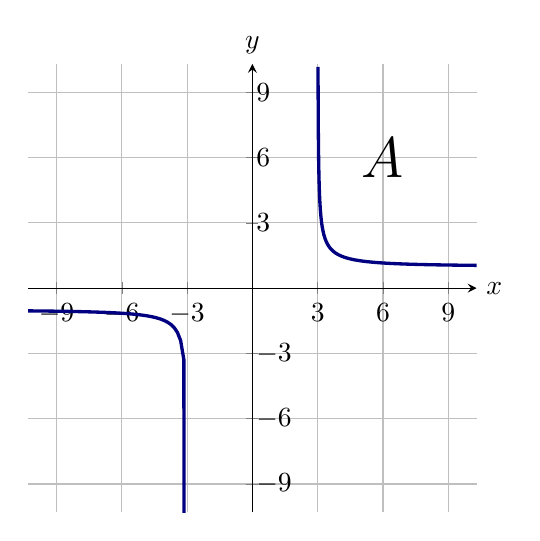
\begin{tikzpicture}
    \begin{axis}[
        xmin=-10.3,xmax=10.3,ymin=-10.3,ymax=10.3,
        clip=true,
        unit vector ratio*=1 1 1,
        axis lines=center,
        grid = major,
        ytick={-21,-18,...,21},
    	xtick={-21,-18,...,21},
        xlabel=$x$, ylabel=$y$,
        y tick label style={anchor=west},
        every axis y label/.style={at=(current axis.above origin),anchor=south},
        every axis x label/.style={at=(current axis.right of origin),anchor=west},
      ]
      \addplot[very thick,penColor,domain=-10.3:-3,samples=50] plot{x/sqrt(x^2-9)};
      \addplot[very thick,penColor,domain=3:10.3,samples=500]  plot{x/sqrt(x^2-9)};

      \node at (axis cs:6,6) {\huge$A$};
      \end{axis}`
  \end{tikzpicture}}
  \resizebox{.3\textwidth}{!}{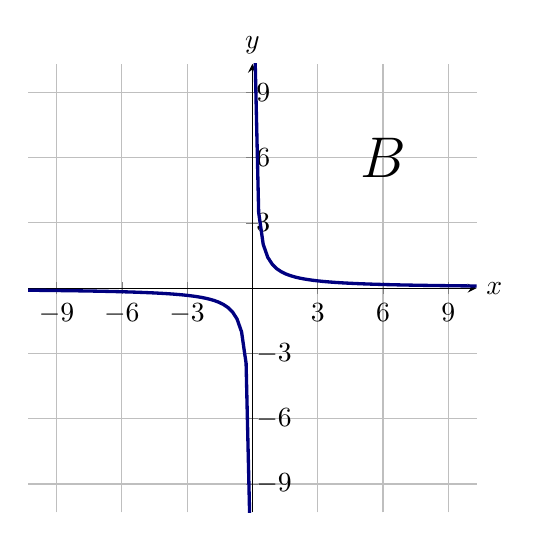
\begin{tikzpicture}
    \begin{axis}[
        xmin=-10.3,xmax=10.3,ymin=-10.3,ymax=10.3,
        clip=true,
        unit vector ratio*=1 1 1,
        axis lines=center,
        grid = major,
        ytick={-21,-18,...,21},
    	xtick={-21,-18,...,21},
        xlabel=$x$, ylabel=$y$,
        y tick label style={anchor=west},
        every axis y label/.style={at=(current axis.above origin),anchor=south},
        every axis x label/.style={at=(current axis.right of origin),anchor=west},
      ]
      \addplot[very thick,penColor,domain=-10.3:-0.08,samples=50] plot{1/x};
      \addplot[very thick,penColor,domain=0.08:10.3,samples=50] plot{1/x};

      \node at (axis cs:6,6) {\huge$B$};
      \end{axis}
  \end{tikzpicture}}
  \\
  \resizebox{.3\textwidth}{!}{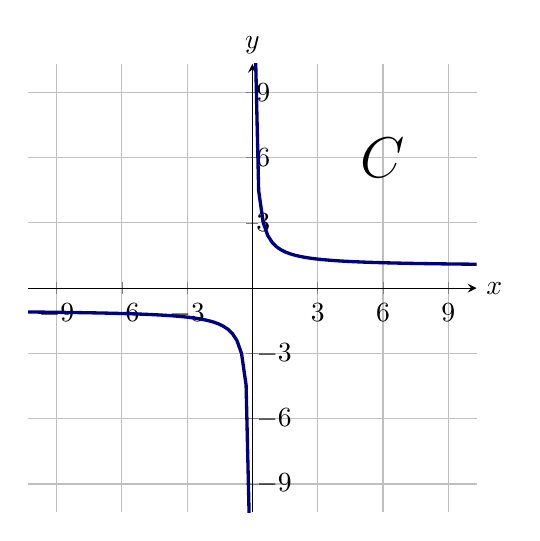
\begin{tikzpicture}
    \begin{axis}[
        xmin=-10.3,xmax=10.3,ymin=-10.3,ymax=10.3,
        clip=true,
        unit vector ratio*=1 1 1,
        axis lines=center,
        grid = major,
        ytick={-21,-18,...,21},
    	xtick={-21,-18,...,21},
        xlabel=$x$, ylabel=$y$,
        y tick label style={anchor=west},
        every axis y label/.style={at=(current axis.above origin),anchor=south},
        every axis x label/.style={at=(current axis.right of origin),anchor=west},
      ]
      \addplot[very thick,penColor,domain=-10.3:-0.08,samples=50] plot{1/x-1};
      \addplot[very thick,penColor,domain=0.08:10.3,samples=50] plot{1/x+1};
      
      \node at (axis cs:6,6) {\huge$C$};
      \end{axis}
  \end{tikzpicture}}
  \resizebox{.3\textwidth}{!}{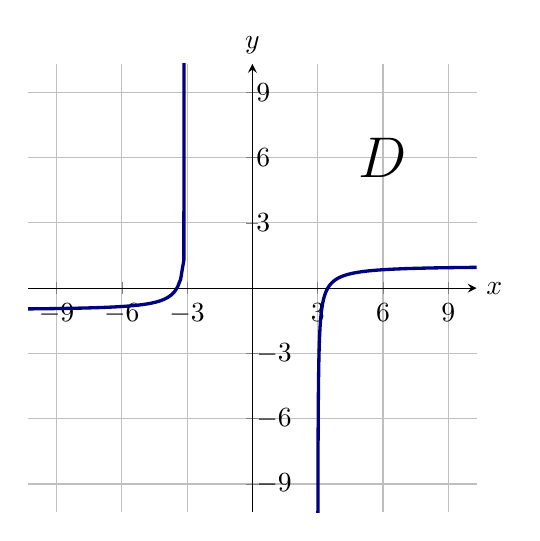
\begin{tikzpicture}
    \begin{axis}[
        xmin=-10.3,xmax=10.3,ymin=-10.3,ymax=10.3,
        clip=true,
        unit vector ratio*=1 1 1,
        axis lines=center,
        grid = major,
        ytick={-21,-18,...,20},
    	xtick={-21,-18,...,20},
        xlabel=$x$, ylabel=$y$,
        y tick label style={anchor=west},
        every axis y label/.style={at=(current axis.above origin),anchor=south},
        every axis x label/.style={at=(current axis.right of origin),anchor=west},
      ]
      \addplot[very thick,penColor,domain=-10.3:-3,samples=50] plot{-x/sqrt(x^2-9)-2};
      \addplot[very thick,penColor,domain=3:10.3,samples=800]  plot{-x/sqrt(x^2-9)+2};
      
      \node at (axis cs:6,6) {\huge$D$};
      \end{axis}
  \end{tikzpicture}}
\end{center}
  
Which graph correctly depicts $f$?
\begin{multipleChoice}
\choice[correct]{$A$}
\choice{$B$}
\choice{$C$}
\choice{$D$}
\end{multipleChoice}

$f$ \wordChoice{\choice[correct]{is}\choice{is not}} one-to-one.

The inverse of $f(x)$ is
\[
f^{-1}(x) = \answer{\frac{3x}{\sqrt{x^2-1}}}.
\]

The domain of $f^{-1}(x)$ (from left to right) is $\left(\answer{-\infty},\answer{-1}\right)\cup\left(\answer{1},\answer{\infty}\right)$.



\end{exercise}
\end{document}
